\subsection{Example query reduction}\label{subsection:background:graphql:example-reduction}

This section contains an example of how the query reduction is made with the help of \textbf{apollo-augmented-hooks} functionality. The client first navigates to a tabular view of all users. This page executes the GraphQL query shown in Listing \ref{code:applied-methods:query-all-users}. After the query is fetched from the GraphQL \ac{API}, the fields in the query are cached inside Apollo's \texttt{InMemoryCache}.

\ifshowListings
\begin{listing}[H]
\begin{minted}{typescript}
query allUsers {
  allUsers {
    id
    username
    email
    password
    firstName
    secondName
    Title { id }
    Salutation { id }
  }
}
\end{minted}
\caption{A GraphQL query to fetch all users.}\label{code:applied-methods:query-all-users}
\end{listing}
\fi

\noindent Afterwards, the client navigates to the detail view of a specific user. The left GraphQL query shown in Figure \ref{fig:applied-methods:comparison-user-reduced-user} is the original query that would normally be fetched from the GraphQL \ac{API} without reducing the query. However, with the help of reducing the query with already existing data, the query on the right is sent to the GraphQL \ac{API}. Exactly the fields which were queried with the GraphQL query shown in Listing \ref{code:applied-methods:query-all-users} are removed. Therefore, 8 of the 16 fields from the query were removed, which reduces the number of queried fields by 50\%. The next chapter goes into more detail, about the impact of reducing queries by utilizing the \texttt{InMemoryCache}.

\ifshowImages
  \begin{figure}[H]
  \centering
  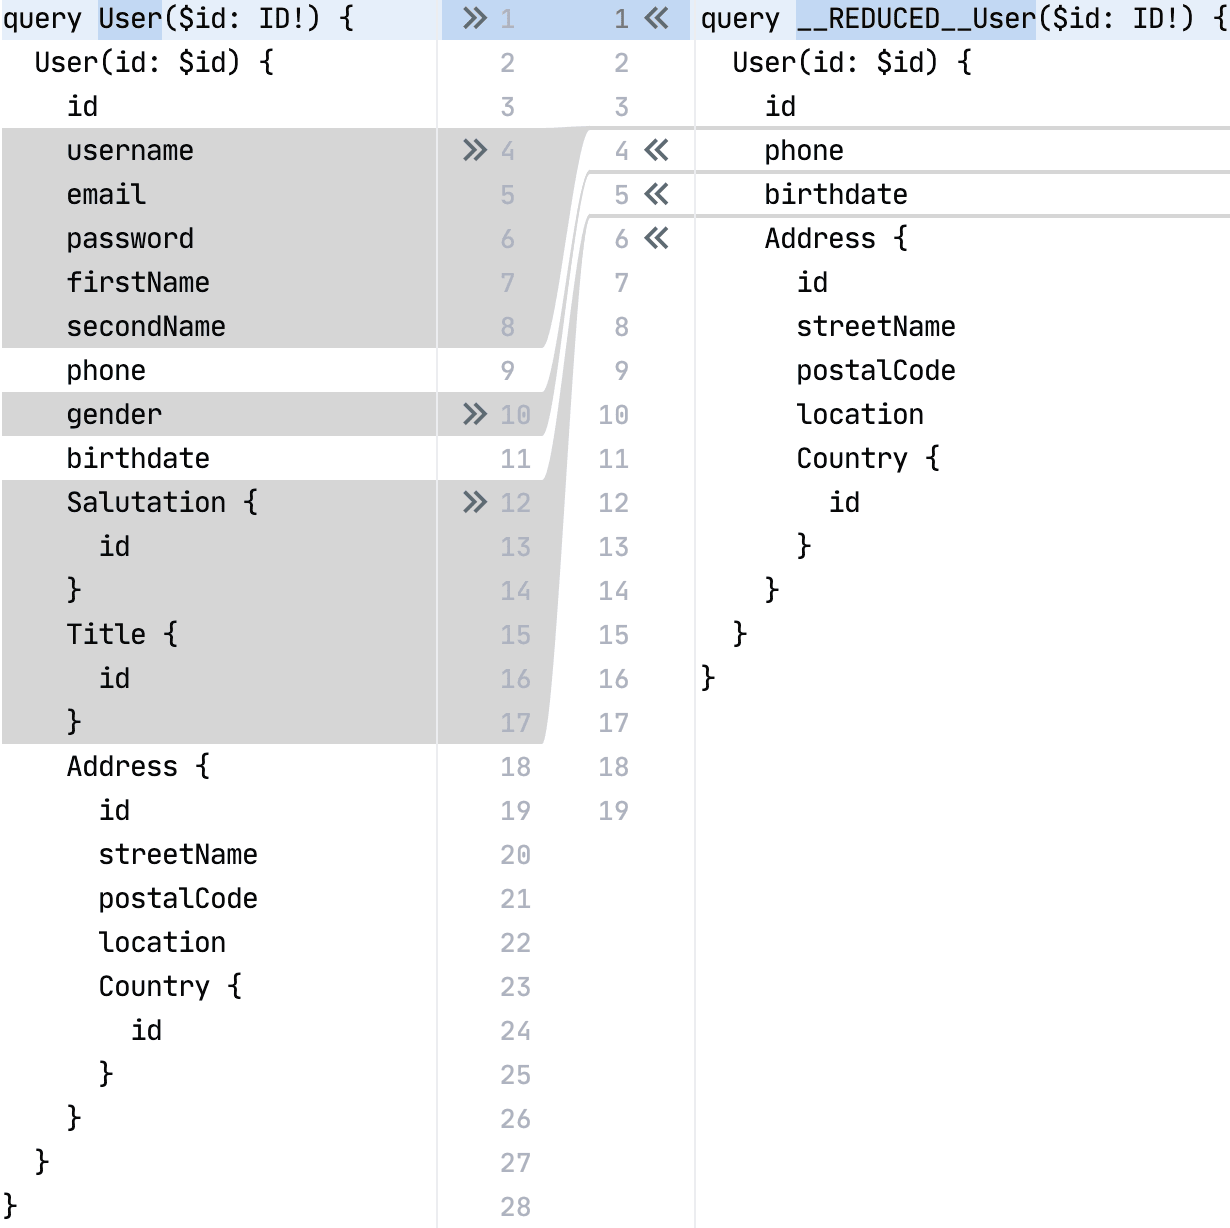
\includegraphics[width=0.65\linewidth]{images/reduction-graphql-examples/compare-user-reduced-user.png}
  \caption{Comparison of the original user- and reduced user-query.}\label{fig:applied-methods:comparison-user-reduced-user}
  \end{figure}
\fi
